\section{トラッカー部}
\label{implement_tracker}
トラッカーノードの実装にはOpenCVを用いる.

QRコードの検出とデコードにはOpenCVに用意されているDetectQRクラスを利用し,そこから得られたQRコードの四角に対してPnPによる3次元再構成を行った.
PnPにはOpenCVに用意されているsolvePnPRansac関数を利用した.

これによりQRコードよりデコードされた次のQRコードの位置情報とQRコードに対するカメラの回転ベクトル,並進ベクトルが得られるのでこれらの情報をナビゲーション部\ref{implement_navigation}にて処理をする

実際にスマートフォン上に表示したQRコードに対して姿勢推定結果を描画したものを以下の図\ref{pnp_qr_img}に示す

\begin{figure}[htbp]
  \begin{center}
    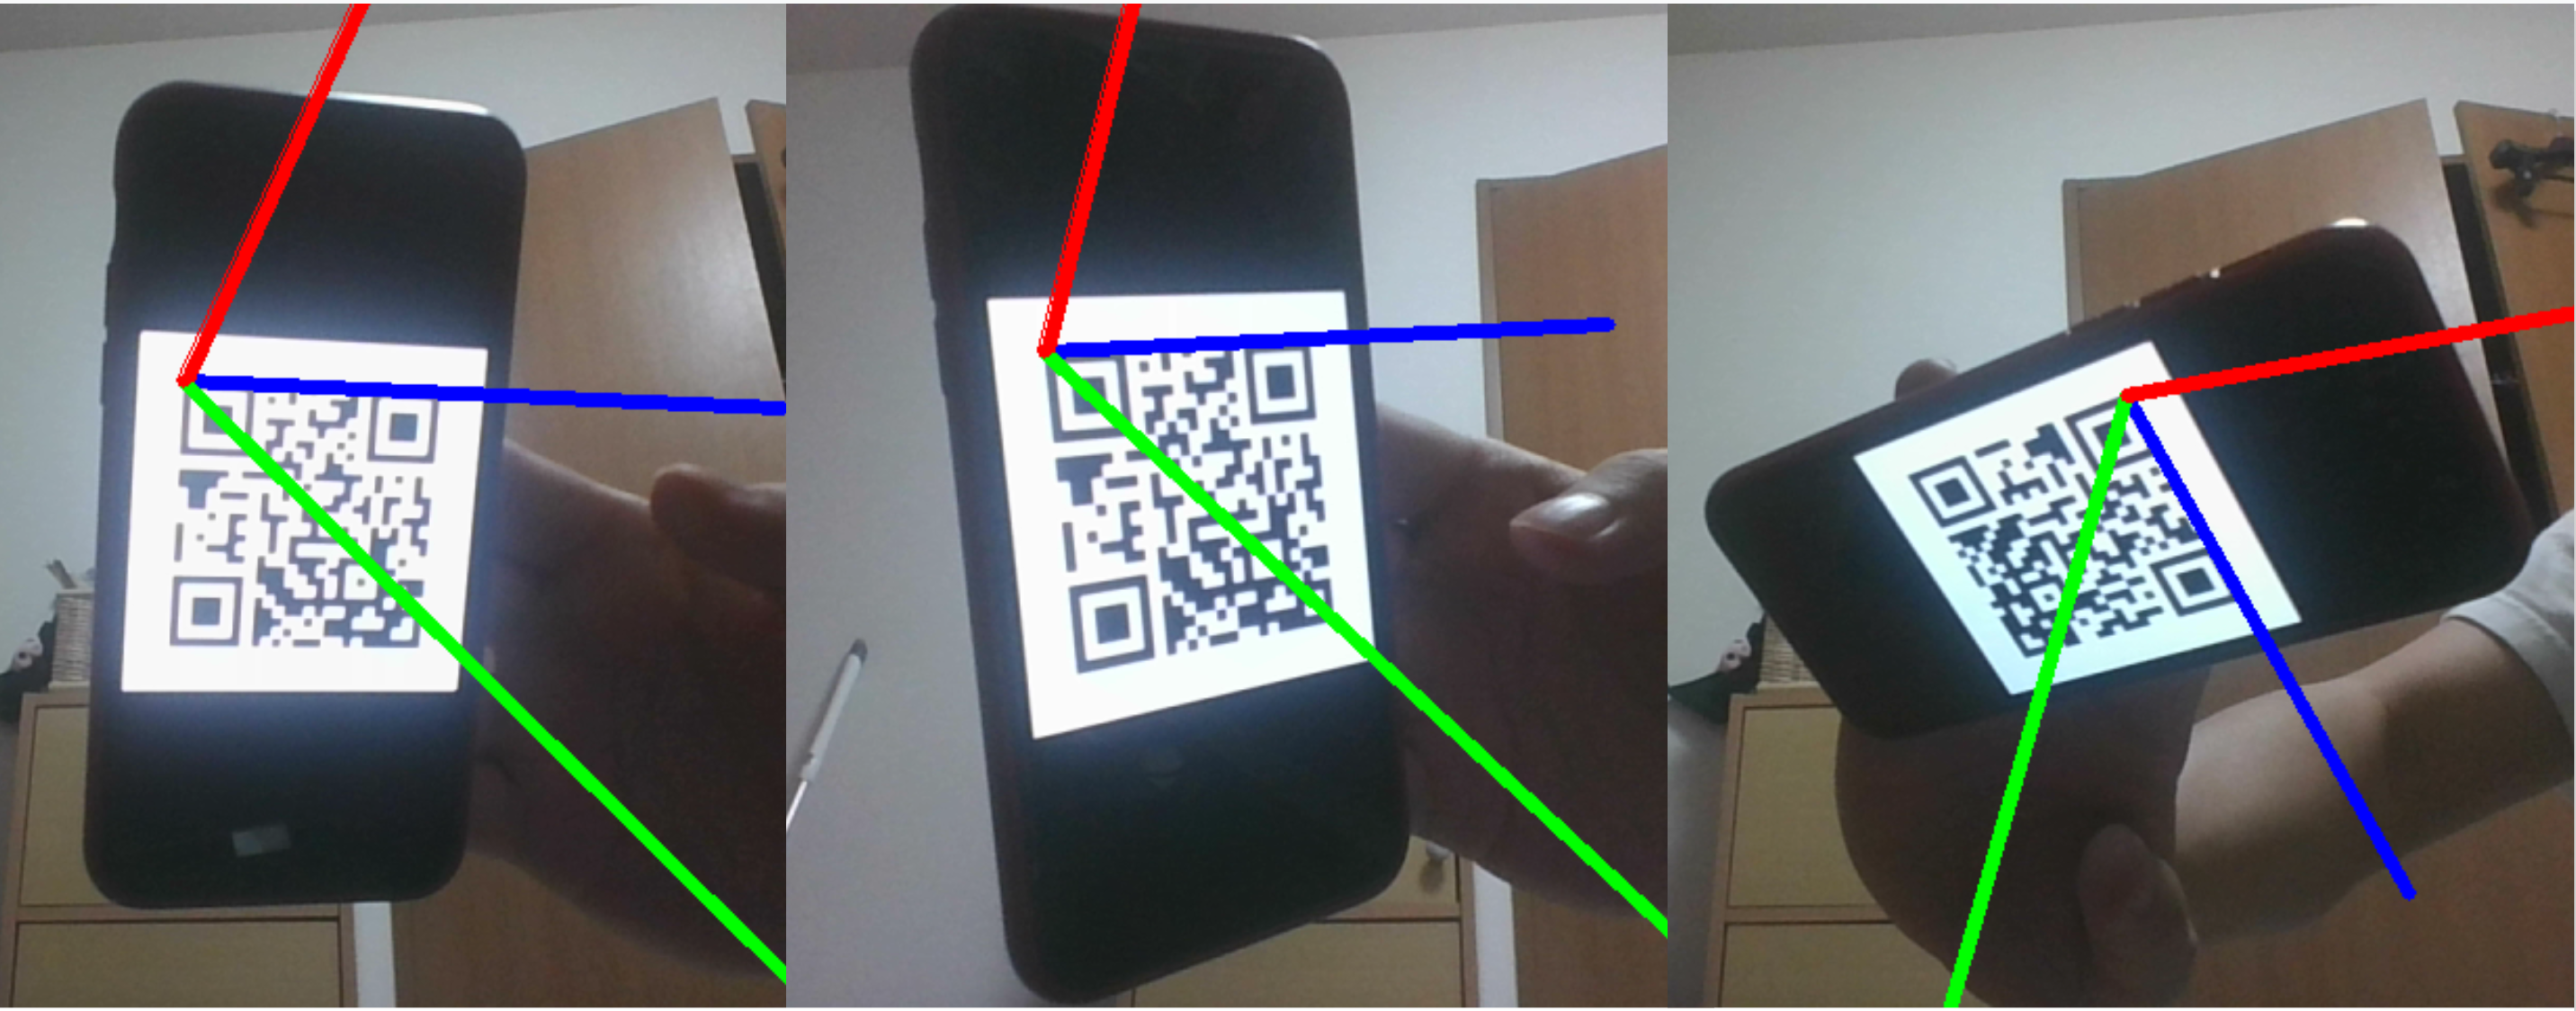
\includegraphics[clip,width=15.0cm]{img/pnp_qr.png}
    \caption{QRコードの姿勢推定結果}
    \label{pnp_qr_img}
  \end{center}
\end{figure}

ソースコードの該当部分をそれぞれ以下のプログラム\ref{src_pnp}に示す.
本コードではQRコードの認識時にノイズが乗る事が多く影響を減らす為に20フレーム分バッファを保持するようにし,
その平均値を用いて制御を行なっている.

\begin{lstlisting}[caption=pnp\_qr.py,label=src_pnp]
def pnp_qr(self, frame):
    img = cv2.cvtColor(frame, cv2.COLOR_RGB2BGR)

    qr = cv2.QRCodeDetector()
    data, points, _ = qr.detectAndDecode(img)
    if data:
        _, origin_rvec, origin_tvec, inliers = cv2.solvePnPRansac(self.objp, points, self.mtx, self.dist)
        if not self.is_moving:
            self.target_pos = json.loads(data)
            tvec = origin_tvec * self.UNIT_SIZE
            rvec = origin_rvec * self.RAD_UNIT
            self.drone_pos_list.append(tvec)
            self.drone_rotate_list.append(rvec)
            if len(self.drone_pos_list) > 20:
                self.drone_pos_list.pop(0)
                self.drone_rotate_list.pop(0)
            drone_avg_pos = np.mean(self.drone_pos_list, axis=(0))
            drone_avg_rotate = np.mean(self.drone_rotate_list, axis=(0))
            self.drone_pos = {
                'x': drone_avg_pos[0],
                'y': drone_avg_pos[1],
                'z': drone_avg_pos[2],
                'r': drone_avg_rotate[1]
            }

        imgpts, jac = cv2.projectPoints(self.axis, origin_rvec, origin_tvec, self.mtx, self.dist)
        img = self.draw(img, points, imgpts)

        cv2.imshow('img',img)
        cv2.waitKey(10)
    else:
        cv2.imshow('img',img)
        cv2.waitKey(10)
\end{lstlisting}
